\documentclass[12pt,a4paper]{article}

% ── Codificación y lenguaje ──────────────────────────────────────────────────
\usepackage[utf8]{inputenc}
\usepackage[T1]{fontenc}
\usepackage[spanish,mexico]{babel}

% ── Fuentes ──────────────────────────────────────────────────────────────────
\usepackage{lmodern}

% ── Márgenes ─────────────────────────────────────────────────────────────────
\usepackage[top=2.5cm, bottom=2.5cm, left=2.5cm, right=2.5cm, headheight=15pt]{geometry}

% ── Colores Institucionales ──────────────────────────────────────────────────
\usepackage{xcolor}
\usepackage{array}

\definecolor{rosado}{RGB}{220, 180, 185}
\definecolor{grisclaro}{RGB}{245, 247, 250}
\definecolor{grisoscuro}{RGB}{50, 50, 60}
\definecolor{azul}{RGB}{30, 70, 120}
\definecolor{verde}{RGB}{39, 130, 80}
\definecolor{vino}{RGB}{120, 30, 50}

% ── Gráficos y TikZ ──────────────────────────────────────────────────────────
\usepackage{graphicx}
\usepackage{tikz}
\usepackage{pgfplots}
\pgfplotsset{compat=1.18}
\usetikzlibrary{calc, positioning, shapes.geometric, arrows.meta, shadows, fit}

% ── Cajas Elegantes (tcolorbox) ─────────────────────────────────────────────
\usepackage{tcolorbox}
\tcbset{colback=grisclaro,colframe=azul!80!black,boxrule=0.8pt,arc=3pt,left=8pt,right=8pt,top=6pt,bottom=6pt,fonttitle=\bfseries}

% ── Código Fuente (Listings) ─────────────────────────────────────────────────
\usepackage{listings}
\lstset{
  basicstyle=\ttfamily\footnotesize,
  backgroundcolor=\color{grisclaro},
  frame=single,
  breaklines=true,
  showstringspaces=false,
  numbers=left,
  numberstyle=\tiny\color{grisoscuro},
  xleftmargin=12pt,
  language=SQL,
  keywordstyle=\color{azul}\bfseries,
  stringstyle=\color{verde},
  commentstyle=\color{grisoscuro}\itshape
}
\lstdefinelanguage{json}{
  basicstyle=\ttfamily\footnotesize,
  morestring=[b]",
  morekeywords={true,false,null},
  keywordstyle=\color{azul}\bfseries,
  stringstyle=\color{verde}
}
\lstdefinelanguage{JavaScript}{
  keywords={const,let,var,function,return,require,async,await,try,catch,new,module,exports,if,else,import,export,default,from,class,extends},
  keywordstyle=\color{azul}\bfseries,
  stringstyle=\color{verde},
  commentstyle=\color{grisoscuro}\itshape,
  morestring=[b]",
  morestring=[b]',
  morestring=[b]`,
  morecomment=[l]{//},
  basicstyle=\ttfamily\footnotesize,
  frame=single,
  backgroundcolor=\color{grisclaro},
  breaklines=true,
  numbers=left,
  numberstyle=\tiny\color{grisoscuro},
  xleftmargin=12pt
}
\lstdefinelanguage{TypeScript}{
  keywords={const,let,var,function,return,require,async,await,try,catch,new,module,exports,if,else,import,export,default,from,class,extends,interface,type,readonly,public,private,protected,Injectable,Controller,Get,Post,Delete,Put,Body,Param,Query,Request,UseGuards,Module,TypeOrmModule},
  keywordstyle=\color{azul}\bfseries,
  stringstyle=\color{verde},
  commentstyle=\color{grisoscuro}\itshape,
  morestring=[b]",
  morestring=[b]',
  morestring=[b]`,
  morecomment=[l]{//},
  basicstyle=\ttfamily\footnotesize,
  frame=single,
  backgroundcolor=\color{grisclaro},
  breaklines=true,
  numbers=left,
  numberstyle=\tiny\color{grisoscuro},
  xleftmargin=12pt
}
\lstdefinelanguage{Python}{
  keywords={def,return,from,import,as,class,async,await,if,else,try,except,raise,with,pass,None,True,False},
  keywordstyle=\color{azul}\bfseries,
  stringstyle=\color{verde},
  commentstyle=\color{grisoscuro}\itshape,
  morestring=[b]",
  morestring=[b]',
  morecomment=[l]{\#},
  basicstyle=\ttfamily\footnotesize,
  frame=single,
  backgroundcolor=\color{grisclaro},
  breaklines=true,
  numbers=left,
  numberstyle=\tiny\color{grisoscuro},
  xleftmargin=12pt
}

% ── Encabezados y Pies de Página ──────────────────────────────────────────────
\usepackage{fancyhdr}
\pagestyle{fancy}
\fancyhf{}
\fancyhead[L]{\small\color{grisoscuro}AOS --- Documentación Final}
\fancyhead[R]{\small\color{grisoscuro}Xiú: Sistema de Reservaciones}
\fancyfoot[C]{\small\thepage}
\renewcommand{\headrulewidth}{0.4pt}

% ── Hipervínculos ────────────────────────────────────────────────────────────
\usepackage[hidelinks]{hyperref}
\urlstyle{same}

% ── Formato de Secciones ─────────────────────────────────────────────────────
\usepackage{titlesec}
\titleformat{\section}{\large\bfseries\color{azul}}{}{0em}{\thesection.\quad}[\vspace{2pt}\hrule\vspace{4pt}]
\titleformat{\subsection}{\normalsize\bfseries\color{vino}}{\thesubsection.}{0.5em}{}
\titleformat{\subsubsection}{\normalsize\bfseries\itshape\color{grisoscuro}}{\thesubsubsection.}{0.5em}{}

% ── Listas y Figuras ─────────────────────────────────────────────────────────
\usepackage{enumitem}
\usepackage{float}
\usepackage{caption}
\captionsetup{font=small,labelfont=bf}

\begin{document}
\pagenumbering{gobble}

% ════════════════════════════════════════════════════════════════════════════
% PORTADA INSTITUCIONAL — UNIVERSIDAD POLITÉCNICA DE PACHUCA
% ════════════════════════════════════════════════════════════════════════════
\begin{titlepage}
\newgeometry{top=2cm,bottom=2cm,left=3.5cm,right=3.5cm}
\begin{tikzpicture}[remember picture,overlay]
  \fill[rosado!80!vino](current page.north east)-- ++(-4.0cm,0)-- ++(0,-5.0cm)--cycle;
  \fill[azul!60](current page.north east)-- ++(-2.0cm,0)-- ++(0,-2.5cm)--cycle;
\end{tikzpicture}
\vspace*{1.0cm}
\begin{center}
  {\Large\scshape\bfseries Universidad Politécnica de Pachuca}\\[4pt]
  {\small\scshape Dirección de Ingeniería en Software}
\end{center}
\vspace{1.8cm}
\begin{center}
  {\Huge\bfseries ARQUITECTURA\\[6pt]ORIENTADA A\\[6pt]SERVICIOS}\\[16pt]
  \rule{0.6\textwidth}{1.5pt}\\[16pt]
  {\Large\bfseries DOCUMENTACIÓN FINAL DEL PROYECTO:}\\[8pt]
  {\LARGE\bfseries\color{vino}Xiú --- Sistema de Reservaciones y Gestión Restaurantera}
\end{center}
\vspace{1.8cm}
\noindent\textbf{DOCENTE:} M. en C. Jazmín Rodríguez Flores\\[8pt]
\noindent\textbf{INTEGRANTES:}\\[4pt]
\noindent\hspace{1cm}$\bullet$ Cristopher Lopez Suarez\\[4pt]
\noindent\hspace{1cm}$\bullet$ Jovanny Hernandez Hernandez\\[8pt]
\noindent\textbf{CARRERA:} Ingeniería en Software\\[8pt]
\noindent\textbf{GRUPO:} 09\_01\\[8pt]
\noindent\textbf{CUATRIMESTRE:} Mayo -- Agosto 2026\\[8pt]
\noindent\textbf{MATERIA:} Arquitectura Orientada a Servicios (AOS)
\vfill
\begin{center}
  \rule{0.8\textwidth}{0.5pt}\\[4pt]
  {\small Pachuca de Soto, Hidalgo, México \quad | \quad 2026}
\end{center}
\end{titlepage}
\restoregeometry

\pagenumbering{arabic}
\tableofcontents
\newpage

% ════════════════════════════════════════════════════════════════════════════
\section{Metodología de Desarrollo y Descripción del Sistema}

\subsection{Defensa y Justificación de la Metodología Ágil (Scrum)}
Para la concepción, diseño e implementación del proyecto \textbf{Xiú --- Sistema de Reservaciones y Gestión Restaurantera}, se adoptó y defendió el marco de trabajo ágil \textbf{Scrum}. Una solución distribuida basada en una \textbf{Arquitectura Orientada a Servicios (SOA)} demanda un proceso de desarrollo iterativo que permita acoplar progresivamente el frontend con múltiples microservicios backend heterogéneos.

A diferencia de los modelos tradicionales rígidos (como Cascada), Scrum facilita la entrega continua de incrementos funcionales de software en **Sprints de 2 semanas**, adaptándose a los cambios de requisitos y proporcionando retroalimentación rápida (Competencia AE2: Aplicar los procesos de desarrollo de software para resolver proyectos que cumplen con los requisitos de los clientes).

\begin{itemize}[leftmargin=*]
  \item \textbf{Organización de Roles en el Proyecto:}
    \begin{itemize}
      \item \textbf{Product Owner / Scrum Master:} Coordinación de la visión del producto, definición de la Definition of Done (DoD) y priorización del backlog.
      \item \textbf{Equipo de Desarrollo (Development Team):} Cristopher Lopez Suarez y Jovanny Hernandez Hernandez, ejecutores de la codificación full-stack, modelado de BD y despliegue en la nube.
    \end{itemize}
  \item \textbf{Artefactos Scrum y Gestión del Tablero Trello:}
    \begin{itemize}
      \item Las Historias de Usuario (HU) y tareas de ingeniería se organizaron y controlaron mediante un tablero **Trello** estructurado en columnas: \textit{Product Backlog}, \textit{Sprint Backlog}, \textit{En Proceso}, \textit{En Revisión / QA} y \textit{Completado}. 
      \item Enlace público al tablero oficial del proyecto: \url{https://trello.com/b/zHsZvXgU/proyecto-final-aos}.
    \end{itemize}
\end{itemize}

\subsection{Funcionalidad General de la Aplicación}
\textbf{Xiú} es una plataforma digital de alta cocina mexicana orientada a optimizar la experiencia gastronómica de los comensales y la eficiencia operativa del personal del restaurante. Sus módulos principales abarcan:

\begin{enumerate}
  \item \textbf{Catálogo Interactivo Gastro-Digital:} Menú de autor con imágenes de alta resolución, precios, alérgenos e ingredientes servidos dinámicamente desde MongoDB Atlas.
  \item \textbf{Seguridad y Autenticación Stateless JWT:} Registro de usuarios y login seguro utilizando tokens **JSON Web Tokens (JWT)** con firma criptográfica HASH-256 y encriptación de contraseñas mediante **Bcrypt** (sal de 10 rondas).
  \item \textbf{Motor Transaccional de Reservaciones:} Sistema de agendado en tiempo real con validación estricta de fecha, horario, número de comensales y capacidad de mesa, garantizando la prevención de doble reservación en MySQL.
  \item \textbf{Tablero Operativo de Mesas (TableBoard Grid):} Visualización interactiva en tiempo real del estado de las mesas del salón mediante un mapa coloreado (Verde = Libre/Disponible, Rojo = Ocupada, Dorado/Amarillo = Reservada) con actualización automática cada 30 segundos.
  \item \textbf{Módulo de Administración NoSQL (CRUD Admin):} Interfaz con control de acceso por rol (\texttt{admin}) para crear, modificar y dar de baja platillos en el catálogo NoSQL.
  \item \textbf{Analítica Gerencial y Generador de Reportes:} Módulo de métricas de ocupación, conteo de reservas confirmadas/canceladas y descarga de datos en formato JSON.
  \item \textbf{Notificaciones de Confirmación por Canales Digitales:} Módulo para enviar la confirmación de cita al teléfono del cliente a través de **WhatsApp** y **SMS**.
\end{enumerate}

\subsection{Listado de Herramientas y Tecnologías Utilizadas}

\begin{center}\small
\begin{tabular}{|l|l|l|p{5.5cm}|}
\hline
\textbf{Categoría} & \textbf{Herramienta} & \textbf{Versión} & \textbf{Propósito en la Arquitectura SOA} \\
\hline
Frontend & React & 18.2.0 & Librería principal para la SPA responsiva en cliente web. \\ \hline
Frontend & Vite & 5.1.0 & Bundler rápido para compilación y empaquetado de assets. \\ \hline
Frontend & React Router DOM & 6.22.0 & Enrutamiento cliente y navegación SPA declarativa. \\ \hline
Frontend & Vanilla CSS3 & N/A & Sistema de diseño personalizado con glassmorphism y tema oscuro. \\ \hline
Backend 1 & Node.js / NestJS & 10.3.0 & Framework progresivo para el microservicio \texttt{auth-service}. \\ \hline
Backend 1 & TypeScript & 5.3.3 & Lenguaje tipado para capas DTO, Controllers y Entidades. \\ \hline
Backend 1 & TypeORM / Passport & 0.3.20 & ORM relacional y middleware de protección con Token JWT. \\ \hline
Backend 2 & FastAPI / Python & 0.110.0 & Framework asíncrono de alto rendimiento para el \texttt{menu-service}. \\ \hline
Backend 2 & Motor / PyMongo & 3.4.0 & Driver ODM asíncrono para interacción con MongoDB Atlas. \\ \hline
Base de Datos & MySQL / PostgreSQL & 8.0 / 15 & Persistencia relacional de usuarios, mesas y reservaciones. \\ \hline
Base de Datos & MongoDB Atlas & 7.0 & Persistencia NoSQL para catálogo flexible de platillos. \\ \hline
Despliegue & Vercel & Cloud & Hosting de producción para el Frontend SPA. \\ \hline
Despliegue & Railway & Cloud & Plataforma PaaS para el microservicio \texttt{auth-service}. \\ \hline
Despliegue & Render & Cloud & Plataforma PaaS para el microservicio \texttt{menu-service}. \\ \hline
Control Versiones & Git / GitHub & N/A & Repositorio distribuido y colaboración por Pull Requests. \\ \hline
Gestión Ágil & Trello & N/A & Tablero Kanban / Scrum para control de Historias de Usuario. \\ \hline
\end{tabular}
\end{center}

% ════════════════════════════════════════════════════════════════════════════
\section{Arquitectura SOA y Diagramas del Sistema}

\subsection{Descripción de la Arquitectura SOA}
El sistema Xiú se basa en una **Arquitectura Orientada a Servicios (SOA)** dividida en microservicios independientes que se comunican mediante contratos **API RESTful HTTP/HTTPS** utilizando formato JSON. Esta arquitectura garantiza alto desacoplamiento, alta cohesión, tolerancia a fallos y escalabilidad independiente de cada servicio.

\begin{figure}[H]
\centering
\begin{tikzpicture}[
  cloud/.style={rectangle, rounded corners=8pt, draw=azul, fill=azul!8, thick, font=\small, align=center, minimum width=3.4cm, minimum height=1.3cm},
  db/.style={rectangle, rounded corners=4pt, draw=vino, fill=vino!8, thick, font=\small, align=center, minimum width=3.0cm, minimum height=1.0cm},
  arr/.style={->, thick, gray}
]
  \node[cloud] (front) at (0,0) {\textbf{Frontend SPA}\\React 18 + Vite\\Desplegado en \textbf{Vercel}};
  \node[cloud] (auth) at (-3.8,-3) {\textbf{Auth-Service (SOA 1)}\\NestJS / TypeScript\\Desplegado en \textbf{Railway}};
  \node[cloud] (menu) at (3.8,-3) {\textbf{Menu-Service (SOA 2)}\\FastAPI / Python\\Desplegado en \textbf{Render}};
  \node[db] (mysql) at (-3.8,-6) {\textbf{MySQL Relacional}\\BD Usuarios / Mesas\\Railway Cloud DB};
  \node[db] (mongo) at (3.8,-6) {\textbf{MongoDB Atlas NoSQL}\\BD Catálogo Platillos\\MongoDB Cloud};

  \draw[arr] (front) -- node[left,font=\tiny]{HTTPS REST / JWT} (auth);
  \draw[arr] (front) -- node[right,font=\tiny]{HTTPS REST / JSON} (menu);
  \draw[arr] (auth) -- node[left,font=\tiny]{SQL (TypeORM)} (mysql);
  \draw[arr] (menu) -- node[right,font=\tiny]{BSON (Motor/ODM)} (mongo);
\end{tikzpicture}
\caption{Diagrama de Despliegue de la Arquitectura SOA en Producción.}
\end{figure}

\subsection{Diagrama de Secuencia: Login y Petición Protegida JWT}

\begin{figure}[H]
\centering
\begin{tikzpicture}[
  node/.style={rectangle, draw=azul, fill=azul!5, minimum width=2.4cm, minimum height=0.7cm, font=\tiny, align=center},
  msg/.style={->, thick, azul!70},
  ret/.style={->, dashed, vino!70}
]
  \node[node] (cli) at (0,0) {Cliente Web\\(Browser)};
  \node[node] (spa) at (3.2,0) {Frontend SPA\\(React)};
  \node[node] (api) at (6.8,0) {Auth-Service\\(NestJS)};
  \node[node] (bd)  at (10.2,0) {Base de Datos\\(MySQL)};

  \draw[msg] (0,-0.7) -- node[above,font=\tiny]{POST /login \{email, pass\}} (3.2,-0.7);
  \draw[msg] (3.2,-1.4) -- node[above,font=\tiny]{POST /api/auth/login} (6.8,-1.4);
  \draw[msg] (6.8,-2.1) -- node[above,font=\tiny]{SELECT * FROM usuarios WHERE email=...} (10.2,-2.1);
  \draw[ret] (10.2,-2.8) -- node[above,font=\tiny]{Retorna registro usuario + hash} (6.8,-2.8);
  \draw[ret] (6.8,-3.5) -- node[above,font=\tiny]{bcrypt.compare() OK $\rightarrow$ Return Token JWT} (3.2,-3.5);
  \draw[ret] (3.2,-4.2) -- node[above,font=\tiny]{localStorage.setItem('token', jwt)} (0,-4.2);

  \draw[msg] (3.2,-5.1) -- node[above,font=\tiny]{GET /api/reservations \{Header Authorization: Bearer JWT\}} (6.8,-5.1);
  \draw[ret] (6.8,-5.8) -- node[above,font=\tiny]{JwtAuthGuard OK $\rightarrow$ 200 OK JSON Data} (3.2,-5.8);
\end{tikzpicture}
\caption{Diagrama de Secuencia del Flujo de Autenticación JWT y Acceso a Servicios.}
\end{figure}

% ════════════════════════════════════════════════════════════════════════════
\section{Listado de Requisitos del Sistema (IEEE 830 y Historias de Usuario)}

\subsection{Requerimientos Funcionales (RF)}

\begin{center}\small
\begin{tabular}{|l|p{3.2cm}|l|p{5.5cm}|}
\hline
\textbf{ID} & \textbf{Nombre} & \textbf{Prioridad} & \textbf{Descripción Funcional} \\
\hline
\textbf{RF-01} & Autenticación y Registro & Alta & Registro e inicio de sesión de usuarios generando tokens JWT firmados. \\ \hline
\textbf{RF-02} & Consulta de Menú NoSQL & Alta & Expone la lista de platillos con imágenes, precios y categorías desde MongoDB. \\ \hline
\textbf{RF-03} & Creación de Reservación & Alta & Registra reservaciones validando capacidad de mesa, fecha y horario no encimado. \\ \hline
\textbf{RF-04} & Confirmación y Notificación & Media & Genera comprobante digital de reserva con opción de notificación WhatsApp/SMS. \\ \hline
\textbf{RF-05} & Cancelación de Reserva & Media & Permite al cliente o admin cancelar una reservación cambiando su estado. \\ \hline
\textbf{RF-06} & Historial de Cliente & Media & Muestra al cliente autenticado sus reservaciones pasadas y activas. \\ \hline
\textbf{RF-07} & CRUD Menú Admin & Alta & Permite al administrador crear, modificar y eliminar platillos en MongoDB. \\ \hline
\textbf{RF-08} & Dashboard del Día & Alta & Muestra al mesero/admin la lista de reservaciones programadas para la fecha. \\ \hline
\textbf{RF-09} & Tablero de Mesas Grid & Alta & Renderiza un esquema visual de mesas clasificadas por colores de ocupación. \\ \hline
\textbf{RF-10} & Generación de Reportes & Media & Permite al administrador filtrar y visualizar métricas de ocupación en JSON. \\ \hline
\textbf{RF-11} & Gestión de Perfil & Baja & Permite ver datos del usuario autenticado y cerrar sesión de forma segura. \\ \hline
\end{tabular}
\end{center}

\subsection{Requerimientos No Funcionales (RNF)}
\begin{itemize}[leftmargin=*]
  \item \textbf{RNF-01 (Seguridad Criptográfica):} Las contraseñas se almacenan encriptadas con algoritmo \texttt{bcrypt} (sal de 10 rondas). Todos los endpoints protegidos requieren el encabezado \texttt{Authorization: Bearer <token\_jwt>}.
  \item \textbf{RNF-02 (Rendimiento):} El tiempo de respuesta de los microservicios backend no supera los 300 ms en condiciones normales de red.
  \item \textbf{RNF-03 (Disponibilidad Cloud):} Los servicios desplegados en Vercel, Railway y Render garantizan un uptime de 99.5\%.
  \item \textbf{RNF-04 (Integridad Relacional):} Restricción de clave única \texttt{(id\_mesa, fecha, hora\_inicio)} en MySQL para prevenir doble reservación en el mismo horario.
  \item \textbf{RNF-05 (Usabilidad Responsive):} Interfaz limpia, responsiva adaptada a dispositivos móviles, tablets y computadoras de escritorio.
  \item \textbf{RNF-06 (Interoperabilidad SOA):} Comunicación estandarizada vía JSON sobre HTTP/HTTPS entre el cliente React y los microservicios NestJS / FastAPI.
\end{itemize}

\subsection{Historias de Usuario (HU) y Asignación en Scrum}

\begin{tcolorbox}[title=HU-01: Autenticación y Registro JWT (Sprint 1)]
\textbf{Prioridad:} Crítica \quad \textbf{Responsable:} Cristopher Lopez Suarez\\
\textbf{Como:} Usuario del sistema\\
\textbf{Quiero:} Registrarme con mis datos e iniciar sesión\\
\textbf{Para:} Obtener mi token de acceso y utilizar las funciones personalizadas\\
\textbf{Criterios de Aceptación:} Encriptar contraseña con bcrypt, generar token JWT válido por 24 horas, validar formato de correo electrónico.
\end{tcolorbox}

\begin{tcolorbox}[title=HU-02: Consultar Menú Interactivo NoSQL (Sprint 1)]
\textbf{Prioridad:} Alta \quad \textbf{Responsable:} Jovanny Hernandez Hernandez\\
\textbf{Como:} Cliente del restaurante\\
\textbf{Quiero:} Explorar el catálogo gastronómico con imágenes y detalles\\
\textbf{Para:} Elegir mis platillos favoritos desde el menú NoSQL\\
\textbf{Criterios de Aceptación:} Consultar la colección \texttt{menu\_items} en MongoDB Atlas, filtrar por categoría (Entradas, Fuertes, Postres, Bebidas).
\end{tcolorbox}

\begin{tcolorbox}[title=HU-03: Creación de Reservaciones con Validación (Sprint 2)]
\textbf{Prioridad:} Crítica \quad \textbf{Responsable:} Cristopher Lopez Suarez\\
\textbf{Como:} Cliente registrado\\
\textbf{Quiero:} Seleccionar fecha, hora, personas y mesa\\
\textbf{Para:} Garantizar mi lugar en el restaurante sin tiempos de espera\\
\textbf{Criterios de Aceptación:} Validar disponibilidad en tiempo real, impedir encimado de reservaciones en la misma mesa y horario.
\end{tcolorbox}

\begin{tcolorbox}[title=HU-04: Confirmación Digital y Notificación WhatsApp/SMS (Sprint 2)]
\textbf{Prioridad:} Media \quad \textbf{Responsable:} Jovanny Hernandez Hernandez\\
\textbf{Como:} Cliente con reserva activa\\
\textbf{Quiero:} Recibir la confirmación de mi reserva vía mensaje digital\\
\textbf{Para:} Conservar comprobante de cita en mi teléfono móvil\\
\textbf{Criterios de Aceptación:} Integración del módulo de envío de mensajes con desglose de datos del cliente, fecha y mesa asignada.
\end{tcolorbox}

\begin{tcolorbox}[title=HU-05 a HU-11: Historias de Usuario Complementarias (Sprints 3--5)]
\textbf{HU-05 --- Cancelar Reservación:} Permitir al cliente o administrador cambiar el estado a ``cancelada''.\\[4pt]
\textbf{HU-06 --- Historial de Cliente:} Vista personalizada con reservaciones pasadas y activas del usuario.\\[4pt]
\textbf{HU-07 --- CRUD de Menú Admin:} Módulo para crear, modificar y eliminar documentos en MongoDB.\\[4pt]
\textbf{HU-08 --- Panel del Día:} Tablero operativo para meseros con reservaciones programadas para la fecha.\\[4pt]
\textbf{HU-09 --- Tablero Gráfico de Mesas (Grid):} Esquema interactivo de mesas por colores (Verde/Rojo/Amarillo).\\[4pt]
\textbf{HU-10 --- Reportes de Ocupación:} Módulo de métricas gerenciales y exportación JSON.\\[4pt]
\textbf{HU-11 --- Perfil del Usuario:} Visualización de datos de la cuenta y cierre de sesión seguro.
\end{tcolorbox}

\subsection{Estimación por Story Points (SP) y Burndown Chart}

\begin{center}\small
\begin{tabular}{|c|p{5.2cm}|c|c|c|}
\hline
\textbf{HU\#} & \textbf{Título de Historia de Usuario} & \textbf{Prioridad} & \textbf{SP} & \textbf{Sprint} \\
\hline
HU-01 & Autenticación y Registro JWT & Crítica & 8 & Sprint 1 \\ \hline
HU-02 & Consultar Menú NoSQL Interactivo & Alta & 5 & Sprint 1 \\ \hline
HU-03 & Crear Reservación con Validación & Crítica & 13 & Sprint 2 \\ \hline
HU-04 & Confirmación y Notificación Digital & Media & 8 & Sprint 2 \\ \hline
HU-05 & Cancelación de Cita por Cliente & Media & 5 & Sprint 3 \\ \hline
HU-06 & Historial de Reservas del Usuario & Media & 5 & Sprint 3 \\ \hline
HU-08 & Panel de Reservaciones del Día & Alta & 8 & Sprint 3 \\ \hline
HU-07 & CRUD de Platillos Admin (MongoDB) & Alta & 13 & Sprint 4 \\ \hline
HU-09 & Tablero Gráfico de Mesas (Grid) & Alta & 13 & Sprint 4 \\ \hline
HU-10 & Generador de Reportes Gerenciales & Media & 8 & Sprint 5 \\ \hline
HU-11 & Perfil del Usuario y Cierre de Sesión & Baja & 3 & Sprint 5 \\ \hline
\multicolumn{3}{|r|}{\textbf{Total Puntos de Historia (Velocity Ideal):}} & \textbf{89 SP} & \\ \hline
\end{tabular}
\end{center}

\begin{figure}[H]
\centering
\begin{tikzpicture}
\begin{axis}[
    title={Gráfica de Quemado (Burndown Chart) --- Proyecto Xiú},
    xlabel={Sprint},
    ylabel={Puntos de Historia Pendientes (SP)},
    xmin=1, xmax=5,
    ymin=0, ymax=95,
    xtick={1,2,3,4,5},
    ytick={0,20,40,60,80,89},
    legend pos=north east,
    ymajorgrids=true,
    grid style=dashed,
    width=0.85\textwidth,
    height=6.0cm
]
\addplot[color=azul,mark=square*,thick] coordinates {(1,89)(2,68)(3,45)(4,19)(5,0)};
\addlegendentry{Propuesto (Ideal)}

\addplot[color=vino,mark=triangle*,ultra thick] coordinates {(1,89)(2,72)(3,43)(4,17)(5,0)};
\addlegendentry{Real Ejecutado}
\end{axis}
\end{tikzpicture}
\caption{Gráfica de Quemado (Burndown Chart) evidenciando el cumplimiento de los 5 Sprints.}
\end{figure}

% ════════════════════════════════════════════════════════════════════════════
\section{Diagrama de Clases del Cliente en Diagrama de Paquetes}

El frontend desarrollado en React 18 SPA se estructuró bajo una arquitectura modular por paquetes de software, garantizando la separación de responsabilidades y facilitando la mantenibilidad.

\subsection{Estructura de Paquetes y Clases del Cliente}

\begin{figure}[H]
\centering
\begin{tikzpicture}[
  package/.style={rectangle, draw=azul, fill=azul!5, thick, font=\tiny, minimum width=5.2cm, align=left, inner sep=5pt}
]
  \node[package] (pages) at (0,3.5) {
    \textbf{package: pages}\\[2pt]
    \textbf{class Home} \{\\
      - heroBgRef: RefObject\\
      + handleScroll(): void\\
    \}\\
    \textbf{class Reservation} \{\\
      - formData: ReservationState\\
      + handleSubmit(e): Promise\\
      + fetchReservations(): void\\
    \}\\
    \textbf{class TableBoard} \{\\
      - mesas: Array<TableState>\\
      + fetchTodayStatus(): void\\
    \}
  };

  \node[package] (comp) at (6.5,3.5) {
    \textbf{package: components}\\[2pt]
    \textbf{class Navbar} \{\\
      + user: UserObject\\
      + logout(): void\\
    \}\\
    \textbf{class TableCard} \{\\
      + mesaId: number\\
      + status: string\\
    \}\\
    \textbf{class MenuCard} \{\\
      + item: MenuItemDoc\\
    \}
  };

  \node[package] (ctx) at (0,0) {
    \textbf{package: context}\\[2pt]
    \textbf{class AuthContext} \{\\
      - user: User\\
      - token: string\\
      + login(email, pass): Promise\\
      + logout(): void\\
    \}
  };

  \node[package] (serv) at (6.5,0) {
    \textbf{package: services}\\[2pt]
    \textbf{class ApiClient} \{\\
      - baseURL: string\\
      + get(url): Promise\\
      + post(url, body): Promise\\
      + sendNotif(phone, msg): Promise\\
    \}
  };

  \draw[->, thick, azul] (pages) -- (comp) node[midway, above, font=\tiny] {renderiza};
  \draw[->, thick, azul] (pages) -- (ctx) node[midway, left, font=\tiny] {consume state};
  \draw[->, thick, azul] (ctx) -- (serv) node[midway, above, font=\tiny] {peticiones HTTP};
  \draw[->, thick, azul] (comp) -- (serv) node[midway, right, font=\tiny] {invoca APIs};
\end{tikzpicture}
\caption{Diagrama de Paquetes y Clases del Cliente React con Atributos y Métodos.}
\end{figure}

\subsection{Explicación de Patrones y Principios de Diseño en el Cliente}
\begin{enumerate}[leftmargin=*]
  \item \textbf{Patrón Context API Provider (React Context):} Se utilizó el patrón Provider en \texttt{AuthContext} para encapsular el estado global de sesión y el Token JWT en el nivel raíz de la aplicación, evitando el antipatrón de ``Prop Drilling''.
  \item \textbf{Patrón Singleton para Cliente HTTP:} El archivo \texttt{services/api.js} exporta una instancia única configurada de Axios que intercepta las peticiones salientes e inyecta dinámicamente el header \texttt{Authorization: Bearer <token>}.
  \item \textbf{Patrón Custom Hook:} Encapsulamiento de lógica mediante \texttt{useAuth()}, permitiendo a cualquier componente acceder a los métodos de sesión de forma desacoplada.
\end{enumerate}

% ════════════════════════════════════════════════════════════════════════════
\section{Diagrama de Clases del Servidor en Diagrama de Paquetes}

El servidor se compone de dos microservicios orientados a servicios (SOA): \texttt{auth-service} (NestJS / TypeScript) y \texttt{menu-service} (FastAPI / Python). Ambos siguen patrones de arquitectura orientada a capas.

\subsection{Estructura de Paquetes y Clases del Servidor}

\begin{figure}[H]
\centering
\begin{tikzpicture}[
  pkg/.style={rectangle, draw=vino, fill=vino!5, thick, font=\tiny, minimum width=5.4cm, align=left, inner sep=5pt}
]
  \node[pkg] (ctrl) at (0,3.5) {
    \textbf{package: controllers}\\[2pt]
    \textbf{class ReservationsController} \{\\
      + create(dto, req): Promise\\
      + findToday(fecha): Promise\\
      + findMine(req): Promise\\
      + updateStatus(id, status): Promise\\
    \}\\
    \textbf{class AuthController} \{\\
      + register(dto): Promise\\
      + login(dto): Promise\\
    \}
  };

  \node[pkg] (serv) at (6.5,3.5) {
    \textbf{package: services}\\[2pt]
    \textbf{class ReservationsService} \{\\
      - repo: Repository<Reservation>\\
      + create(dto, userId): Reservation\\
      + getAvailableTables(f, h, p): Table[]\\
      + updateStatus(id, estado): void\\
    \}\\
    \textbf{class AuthService} \{\\
      + validateUser(e, p): User\\
    \}
  };

  \node[pkg] (dto) at (0,0) {
    \textbf{package: dto / guards}\\[2pt]
    \textbf{class CreateReservationDto} \{\\
      + id\_mesa: number\\
      + fecha: string\\
      + hora\_inicio: string\\
      + num\_personas: number\\
    \}\\
    \textbf{class JwtAuthGuard} \{\\
      + canActivate(context): boolean\\
    \}
  };

  \node[pkg] (ent) at (6.5,0) {
    \textbf{package: entities / models}\\[2pt]
    \textbf{class Reservation} \{\\
      + id\_reservacion: number\\
      + id\_usuario: number\\
      + id\_mesa: number\\
      + estado: string\\
    \}\\
    \textbf{class MenuItem (Mongo)} \{\\
      + \_id: ObjectId\\
      + nombre: string\\
    \}
  };

  \draw[->, thick, vino] (ctrl) -- (serv) node[midway, above, font=\tiny] {inyecta};
  \draw[->, thick, vino] (ctrl) -- (dto) node[midway, left, font=\tiny] {valida};
  \draw[->, thick, vino] (serv) -- (ent) node[midway, above, font=\tiny] {persiste};
\end{tikzpicture}
\caption{Diagrama de Paquetes y Clases del Servidor (NestJS + FastAPI) con Atributos y Métodos.}
\end{figure}

\subsection{Explicación de Patrones y Principios de Diseño en el Servidor}
\begin{enumerate}[leftmargin=*]
  \item \textbf{Patrón DTO (Data Transfer Object):} Implementado mediante clases TypeScript (\texttt{CreateReservationDto}) decoradas con \texttt{class-validator} (\texttt{@IsNotEmpty()}, \texttt{@IsString()}, \texttt{@IsInt()}). Garantiza el tipado y filtrado de datos antes de ingresar a la capa del servicio.
  \item \textbf{Patrón Repository (TypeORM):} En NestJS, la comunicación con MySQL abstrae el SQL mediante el repositorio inyectado (\texttt{@InjectRepository(Reservation)}), aislando las operaciones de BD de la lógica de negocio.
  \item \textbf{Patrón Decorador y Guard Interceptor:} El decorador \texttt{@UseGuards(JwtAuthGuard, RolesGuard)} valida el token JWT de las peticiones HTTP y verifica los permisos por rol (\texttt{@Roles('admin')}).
  \item \textbf{Inyección de Dependencias (DI):} El contenedor IoC de NestJS provee automáticamente las instancias de los servicios a los controladores a través de sus constructores.
\end{enumerate}

% ════════════════════════════════════════════════════════════════════════════
\section{Modelo de Datos y Persistencia Híbrida (BD Relacional + NoSQL)}

El sistema utiliza una **persistencia políglota (Polyglot Persistence)** para responder con eficiencia a los requerimientos de cada módulo.

\subsection{Modelo Relacional (MySQL / PostgreSQL)}
Maneja el núcleo de usuarios, disponibilidad de mesas y transacciones de reservaciones.

\subsubsection{Diagrama Entidad-Relación (E-R)}

\begin{figure}[H]
\centering
\begin{tikzpicture}[
  table/.style={rectangle, draw=azul, fill=grisclaro, thick, font=\footnotesize, align=left, inner sep=4pt}
]
  \node[table] (usr) {
    \textbf{usuarios (MySQL)}\\[2pt]
    \underline{id\_usuario} : INT (PK)\\
    nombre : VARCHAR(100)\\
    email : VARCHAR(150) (UQ)\\
    password\_hash : VARCHAR(255)\\
    rol : ENUM('cliente','mesero','admin')\\
    activo : BOOLEAN
  };

  \node[table, right=0.9cm of usr] (res) {
    \textbf{reservaciones (MySQL)}\\[2pt]
    \underline{id\_reservacion} : INT (PK)\\
    id\_usuario : INT (FK)\\
    id\_mesa : INT (FK)\\
    fecha : DATE\\
    hora\_inicio : TIME\\
    num\_personas : INT\\
    estado : VARCHAR(20)
  };

  \node[table, right=0.9cm of res] (mesa) {
    \textbf{mesas (MySQL)}\\[2pt]
    \underline{id\_mesa} : INT (PK)\\
    numero : INT (UQ)\\
    capacidad : INT\\
    activa : BOOLEAN
  };

  \draw[->, thick, azul] (usr) -- (res) node[midway, above, font=\tiny] {1:N};
  \draw[->, thick, azul] (mesa) -- (res) node[midway, above, font=\tiny] {1:N};
\end{tikzpicture}
\caption{Modelo Entidad-Relación de la Base de Datos Relacional.}
\end{figure}

\subsection{Modelo NoSQL (MongoDB Atlas Document Store)}
Para el catálogo dinámico de alimentos se utiliza **MongoDB Atlas**. Permite estructurar platillos con arreglos de ingredientes, etiquetas y alérgenos sin requerir tablas intermedias de uniones relacionales.

\subsubsection{Modelo de Documentos BSON / JSON (Explicación de Tuplas/Campos)}

\begin{lstlisting}[language=json, caption={Documento NoSQL en MongoDB Atlas para menu\_items}]
{
  "_id": { "$oid": "665abc123def000000000001" },
  "nombre": "Tacos de Sirloin al Pastor",
  "descripcion": "3 tacos marinados en achiote artesanal con pina asada",
  "categoria": "Platillo Principal",
  "precio": 185.00,
  "imagen_url": "https://restaurante-frontend-omega.vercel.app/img/tacos.jpg",
  "disponible": true,
  "ingredientes": ["sirloin", "achiote", "pina", "tortilla de maiz"],
  "alergenos": ["gluten"],
  "opciones": [
    { "nombre": "Sin cebolla", "costo_extra": 0.00 },
    { "nombre": "Extra queso", "costo_extra": 15.00 }
  ],
  "tiempo_preparacion_min": 15
}
\end{lstlisting}

\subsection{Evidencia de Creación y Modificación mediante Servicios SOA}
El sistema demuestra persistencia activa a través de sus microservicios:
\begin{enumerate}
  \item \textbf{Inserción y Edición Relacional (MySQL):} La invocación de \texttt{POST /api/reservations} realiza la validación e inserción de la tupla en la tabla \texttt{reservaciones}. La actualización de estado (\texttt{PUT /api/reservations/:id/status}) modifica el atributo \texttt{estado}.
  \item \textbf{Inserción y Edición NoSQL (MongoDB):} El servicio \texttt{menu-service} expone endpoints \texttt{POST /api/v1/menu} y \texttt{PUT /api/v1/menu/:id} para insertar y editar documentos BSON directamente en el clúster cloud de MongoDB Atlas.
\end{enumerate}

% ════════════════════════════════════════════════════════════════════════════
\section{Pruebas del Cliente (Formato IEEE 829)}

Las pruebas cliente se planificaron y ejecutaron de acuerdo con el estándar **IEEE 829-1998**.

\begin{tcolorbox}[title=Prueba Cliente 01: Registro e Inicio de Sesión JWT]
\textbf{Identificador:} TC-CLIENT-01\\[2pt]
\textbf{Elemento de Prueba:} Componentes de Autenticación (\texttt{Login.jsx} / \texttt{Register.jsx})\\[2pt]
\textbf{Objetivo:} Confirmar que un usuario puede autenticarse y guardar el Token JWT en el cliente de forma transparente.\\[2pt]
\textbf{Entorno de Prueba:} Google Chrome v122 en entorno de producción Vercel.\\[2pt]
\textbf{Datos de Entrada:} Email: \texttt{cliente.test@xiu.mx}, Password: \texttt{Password123!}\\[2pt]
\textbf{Pasos Ejecutados:}
\begin{enumerate}[leftmargin=1.5em, topsep=2pt, itemsep=0pt]
  \item Ingresar a la URL de login y capturar credenciales.
  \item Enviar formulario y esperar respuesta del microservicio.
\end{enumerate}
\textbf{Resultado Esperado:} Código HTTP 200 OK con el token JWT. El cliente guarda el token en \texttt{localStorage} y muestra el Navbar autenticado.\\[2pt]
\textbf{Resultado Actual:} Éxito. Token recibido, guardado en \texttt{localStorage} y sesión iniciada. \textbf{[PASÓ]}
\end{tcolorbox}
\vspace{0.2cm}

\begin{tcolorbox}[title=Prueba Cliente 02: Validación de Formulario de Reservación]
\textbf{Identificador:} TC-CLIENT-02\\[2pt]
\textbf{Elemento de Prueba:} Componente de Reservas (\texttt{Reservation.jsx})\\[2pt]
\textbf{Objetivo:} Verificar que la interfaz cliente intercepte e impida envíos de reservación con campos vacíos.\\[2pt]
\textbf{Entorno de Prueba:} Navegador Web en Laptop y Móvil.\\[2pt]
\textbf{Datos de Entrada:} Formulario sin fecha ni hora seleccionada.\\[2pt]
\textbf{Pasos Ejecutados:} (1) Ir a \texttt{/reservations}. (2) Presionar ``Confirmar Reserva'' sin llenar fecha.\\[2pt]
\textbf{Resultado Esperado:} Intercepción inmediata en el cliente mostrando advertencias en rojo.\\[2pt]
\textbf{Resultado Actual:} Éxito. Las alertas de validación impidieron la petición HTTP innecesaria. \textbf{[PASÓ]}
\end{tcolorbox}
\vspace{0.2cm}

\begin{tcolorbox}[title=Prueba Cliente 03: Tablero Interactivo de Mesas por Colores]
\textbf{Identificador:} TC-CLIENT-03\\[2pt]
\textbf{Elemento de Prueba:} Componente de Mapa de Mesas (\texttt{TableBoard.jsx})\\[2pt]
\textbf{Objetivo:} Confirmar que la cuadrícula de mesas renderice dinámicamente su ocupación por colores.\\[2pt]
\textbf{Entorno de Prueba:} Navegador Chrome en resolución 1920x1080.\\[2pt]
\textbf{Pasos Ejecutados:} (1) Iniciar sesión como \texttt{admin} o \texttt{mesero}. (2) Navegar a \texttt{/tableboard}.\\[2pt]
\textbf{Resultado Esperado:} Renderizado del grid con 12 mesas. Verde = Libre, Rojo = Ocupada, Dorado = Reservada.\\[2pt]
\textbf{Resultado Actual:} Éxito. El tablero sincronizó los estados visualmente en tiempo real. \textbf{[PASÓ]}
\end{tcolorbox}
\vspace{0.2cm}

\begin{tcolorbox}[title=Prueba Cliente 04: Confirmación Digital vía WhatsApp/SMS]
\textbf{Identificador:} TC-CLIENT-04\\[2pt]
\textbf{Elemento de Prueba:} Componente de Notificaciones (\texttt{Profile.jsx})\\[2pt]
\textbf{Objetivo:} Probar la activación del botón de envío de confirmación de reserva al celular del usuario.\\[2pt]
\textbf{Entorno de Prueba:} Navegador Web Desktop.\\[2pt]
\textbf{Pasos Ejecutados:} (1) Ir a \texttt{/profile}. (2) Ingresar número móvil. (3) Clic en ``WhatsApp''.\\[2pt]
\textbf{Resultado Esperado:} Redirección a WhatsApp Web con el mensaje formateado de la cita.\\[2pt]
\textbf{Resultado Actual:} Éxito. La app abrió el enlace prellenado correctamente. \textbf{[PASÓ]}
\end{tcolorbox}

% ════════════════════════════════════════════════════════════════════════════
\section{Pruebas del Servidor (Formato IEEE 829)}

Las pruebas de los microservicios backend evalúan los endpoints RESTful, validaciones DTO y la protección JWT bajo el estándar **IEEE 829-1998**.

\begin{tcolorbox}[title=Prueba Servidor 01: Creación de Reservación (HTTP 201 Created)]
\textbf{Identificador:} TC-SERVER-01\\[2pt]
\textbf{Endpoint / Servicio:} \texttt{POST /api/reservations} (\texttt{auth-service} NestJS)\\[2pt]
\textbf{Objetivo:} Validar la creación transaccional e inserción en MySQL de una reservación válida.\\[2pt]
\textbf{JSON Body de Entrada:}
\begin{lstlisting}[language=json]
{
  "id_mesa": 2,
  "fecha": "2026-08-15",
  "hora_inicio": "14:00:00",
  "num_personas": 4
}
\end{lstlisting}
\textbf{Resultado Esperado:} Código HTTP \textbf{201 Created} y objeto JSON con el ID de reserva asignado.\\[2pt]
\textbf{Resultado Actual:} Éxito. El servicio registró la reserva en la BD relacional y retornó status 201. \textbf{[PASÓ]}
\end{tcolorbox}
\vspace{0.2cm}

\begin{tcolorbox}[title=Prueba Servidor 02: Rechazo de Horarios Encimados (HTTP 400 Bad Request)]
\textbf{Identificador:} TC-SERVER-02\\[2pt]
\textbf{Endpoint / Servicio:} \texttt{POST /api/reservations} (\texttt{auth-service} NestJS)\\[2pt]
\textbf{Objetivo:} Validar que el servidor bloquee la duplicidad de reservas en la misma mesa y horario.\\[2pt]
\textbf{JSON Body de Entrada:} Mismo payload de la prueba TC-SERVER-01.\\[2pt]
\textbf{Resultado Esperado:} Código HTTP \textbf{400 Bad Request} o \textbf{409 Conflict}.\\[2pt]
\textbf{Resultado Actual:} Éxito. El backend interceptó el conflicto e impidió la doble reserva. \textbf{[PASÓ]}
\end{tcolorbox}
\vspace{0.2cm}

\begin{tcolorbox}[title=Prueba Servidor 03: Consulta NoSQL del Menú (HTTP 200 OK)]
\textbf{Identificador:} TC-SERVER-03\\[2pt]
\textbf{Endpoint / Servicio:} \texttt{GET /api/v1/menu} (\texttt{menu-service} FastAPI)\\[2pt]
\textbf{Objetivo:} Probar la lectura de los documentos de platillos almacenados en MongoDB Atlas.\\[2pt]
\textbf{Resultado Esperado:} Código HTTP \textbf{200 OK} y arreglo JSON de platillos.\\[2pt]
\textbf{Resultado Actual:} Éxito. La respuesta fue entregada en 110 ms con la lista de platillos. \textbf{[PASÓ]}
\end{tcolorbox}
\vspace{0.2cm}

\begin{tcolorbox}[title=Prueba Servidor 04: Protección de Endpoint Sin Token (HTTP 401 Unauthorized)]
\textbf{Identificador:} TC-SERVER-04\\[2pt]
\textbf{Endpoint / Servicio:} \texttt{GET /api/reservations/my} (\texttt{auth-service} NestJS)\\[2pt]
\textbf{Objetivo:} Verificar que un endpoint protegido por \texttt{JwtAuthGuard} rechace peticiones sin header JWT.\\[2pt]
\textbf{Resultado Esperado:} Código HTTP \textbf{401 Unauthorized}.\\[2pt]
\textbf{Resultado Actual:} Éxito. El guard denegó el acceso protegiendo la información. \textbf{[PASÓ]}
\end{tcolorbox}

% ════════════════════════════════════════════════════════════════════════════
\section{Evidencia Visual del Funcionamiento y Base de Datos}

A continuación se presentan las evidencias visuales del sistema desplegado y su infraestructura de base de datos:

\subsection{Interfaz Principal y Menú NoSQL}
La figura \ref{fig:cap_home} muestra la página de inicio desplegada en Vercel.

\begin{figure}[H]
\centering
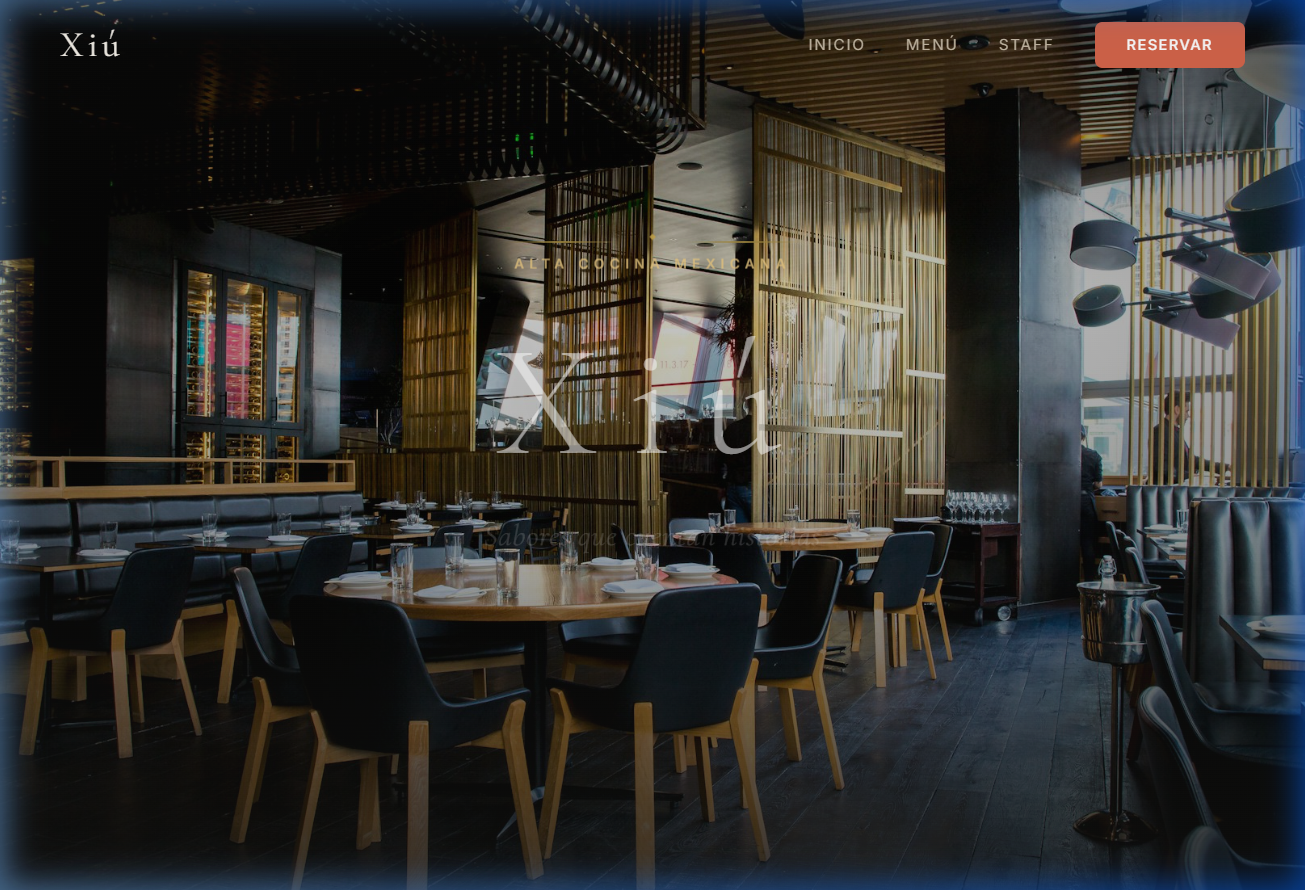
\includegraphics[width=0.88\textwidth]{img/home.png}
\caption{Interfaz Principal (SPA React) desplegada en Vercel.}
\label{fig:cap_home}
\end{figure}

\subsection{Módulo de Autenticación}
La figura \ref{fig:cap_login} muestra el formulario de autenticación JWT.

\begin{figure}[H]
\centering
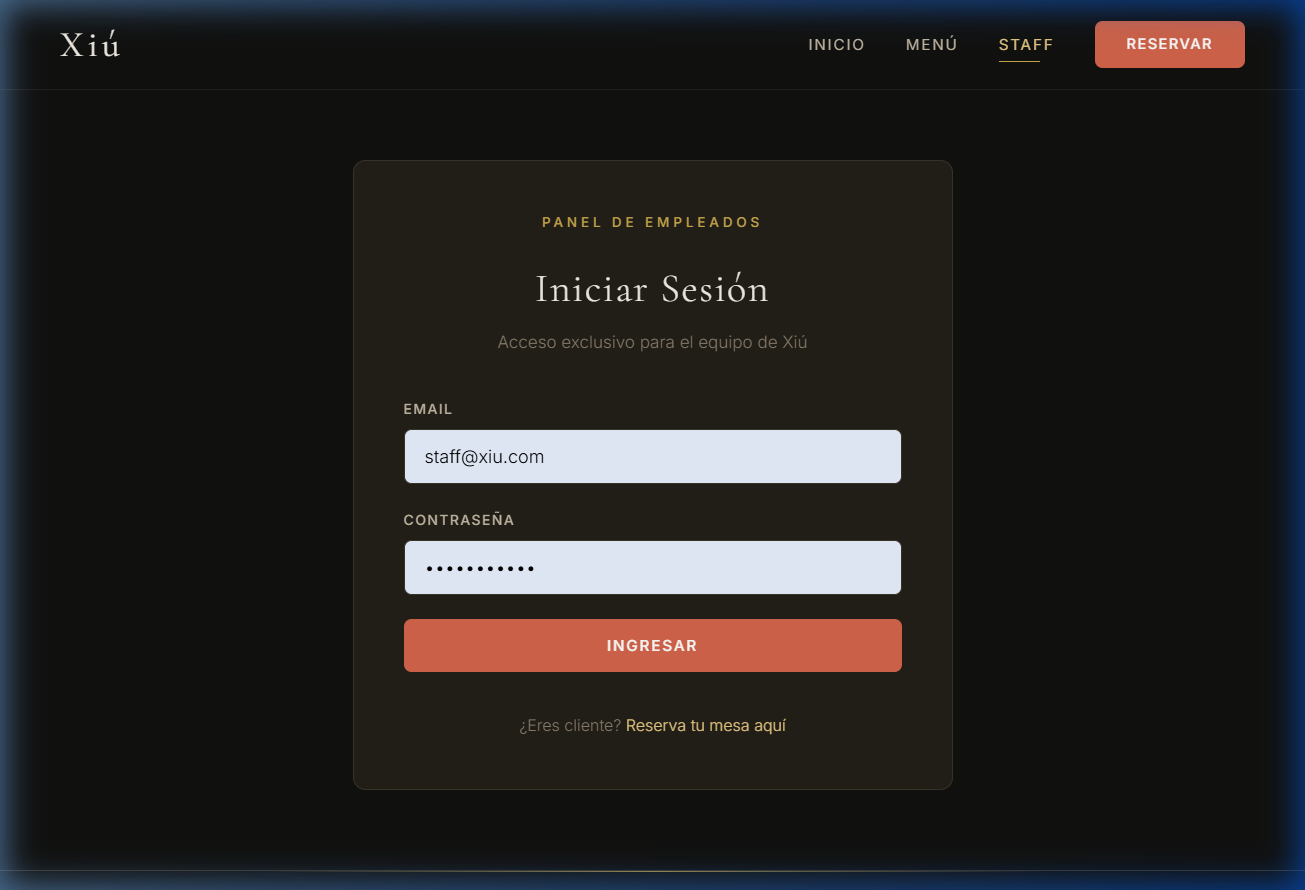
\includegraphics[width=0.72\textwidth]{img/login.png}
\caption{Módulo de Autenticación de Usuarios.}
\label{fig:cap_login}
\end{figure}

\subsection{Módulo de Reservaciones}
Las figuras \ref{fig:cap_res1} y \ref{fig:cap_res2} presentan el flujo de agendado y confirmación.

\begin{figure}[H]
\centering
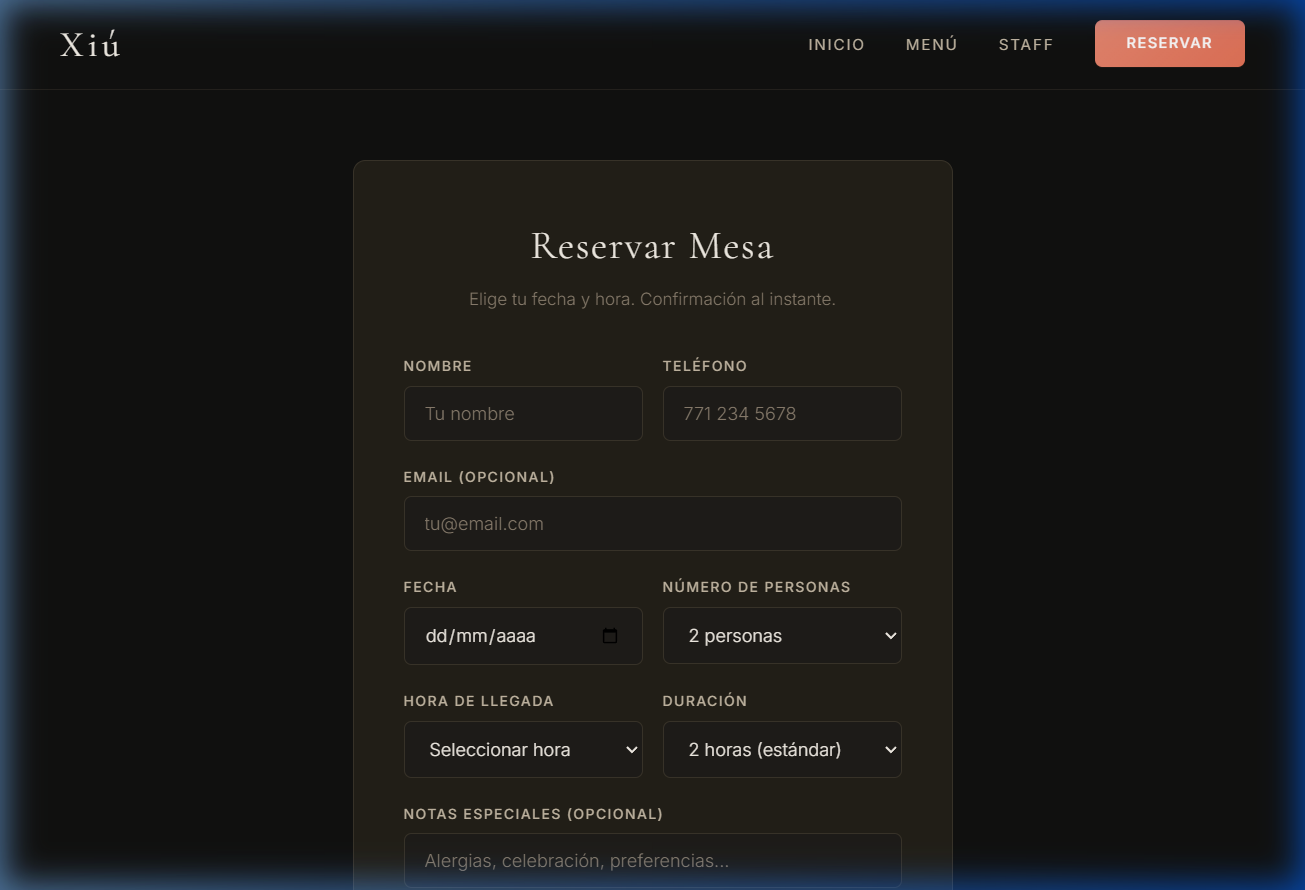
\includegraphics[width=0.85\textwidth]{img/reservacion.png}
\caption{Formulario de Reservación de Mesas.}
\label{fig:cap_res1}
\end{figure}

\begin{figure}[H]
\centering
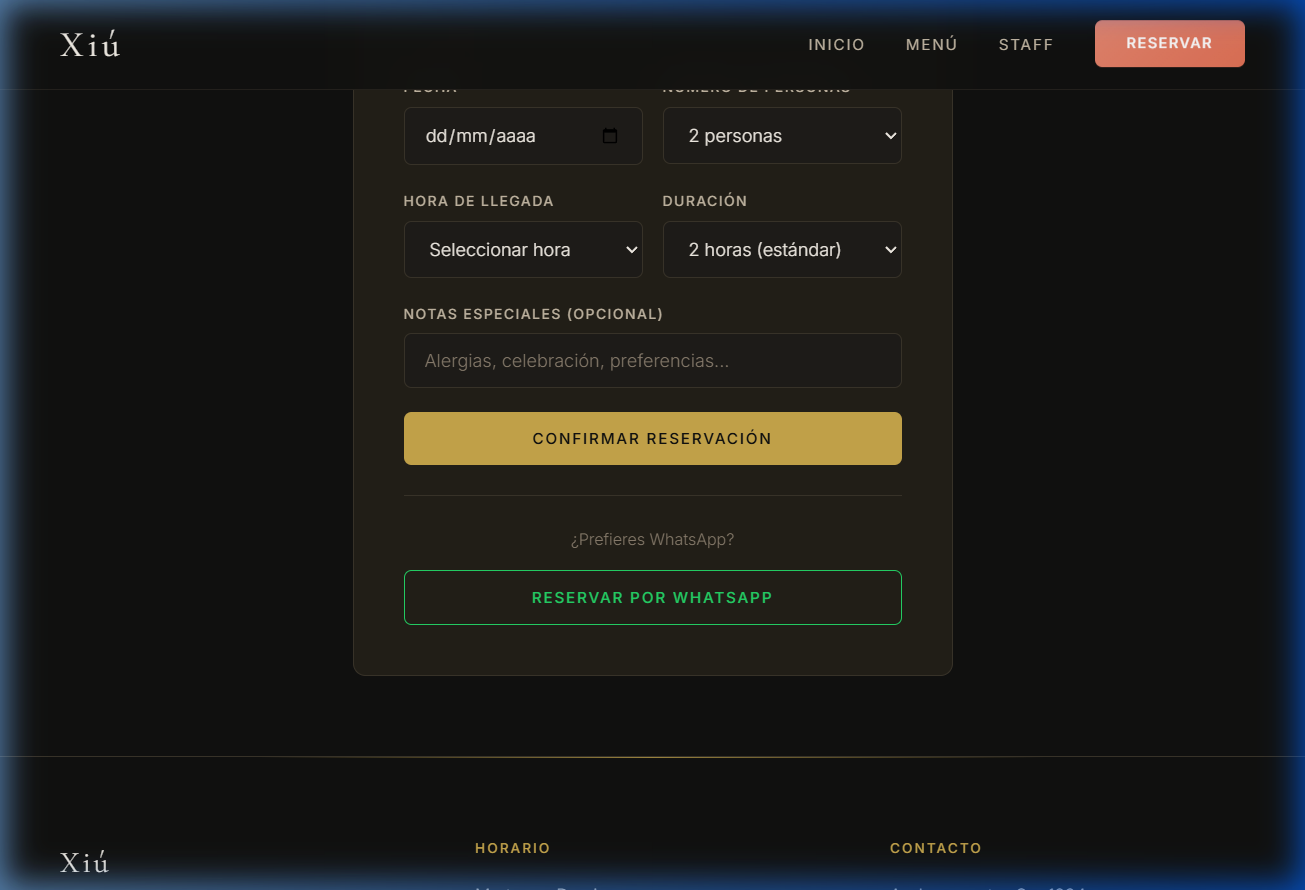
\includegraphics[width=0.85\textwidth]{img/reservacion_scroll.png}
\caption{Confirmación de Reservación.}
\label{fig:cap_res2}
\end{figure}

\subsection{Persistencia Relacional}
Las figuras \ref{fig:cap_sql1} y \ref{fig:cap_sql2} comprueban las tablas creadas e información en la BD relacional.

\begin{figure}[H]
\centering
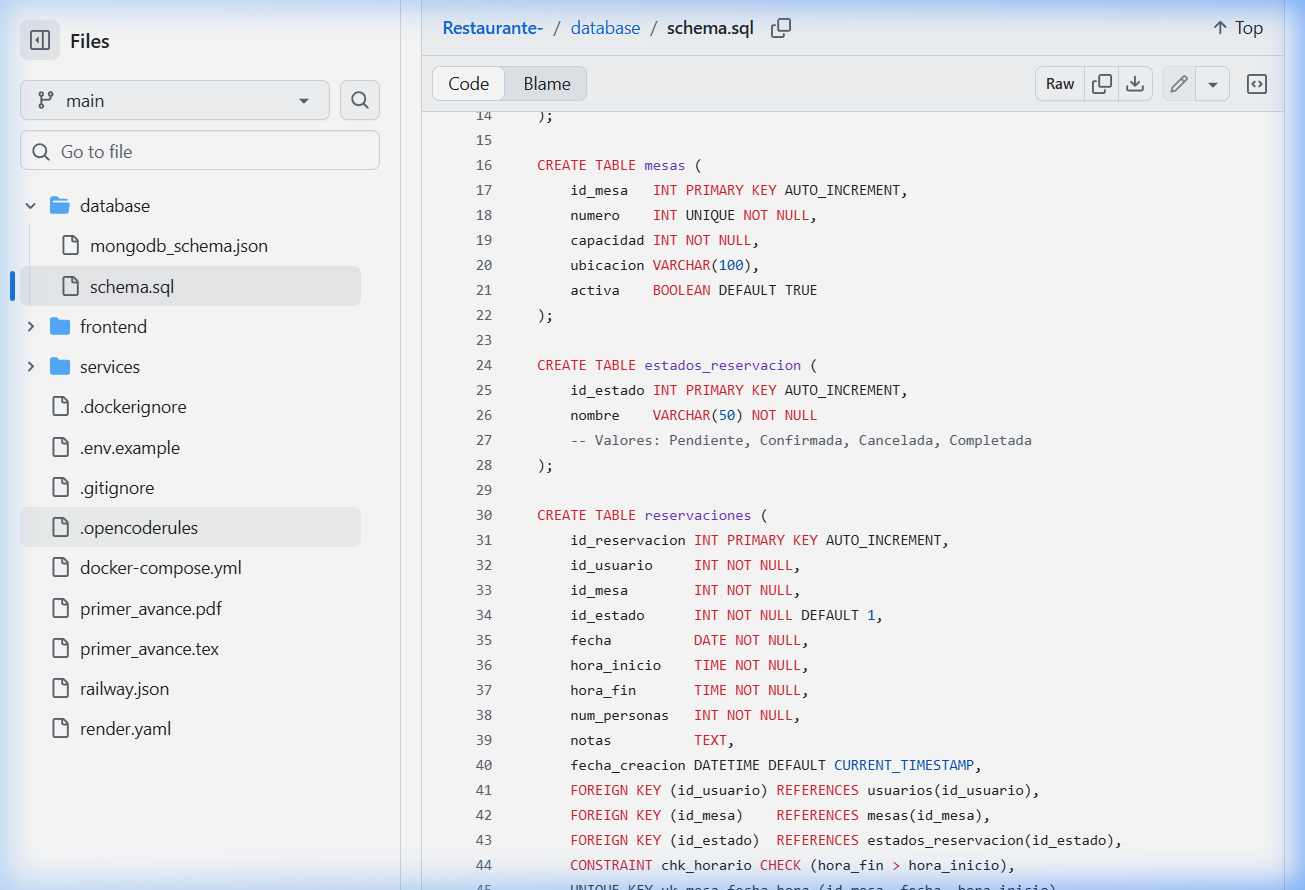
\includegraphics[width=0.85\textwidth]{img/schema_sql1.png}
\caption{Estructura de tablas en la Base de Datos Relacional.}
\label{fig:cap_sql1}
\end{figure}

\begin{figure}[H]
\centering
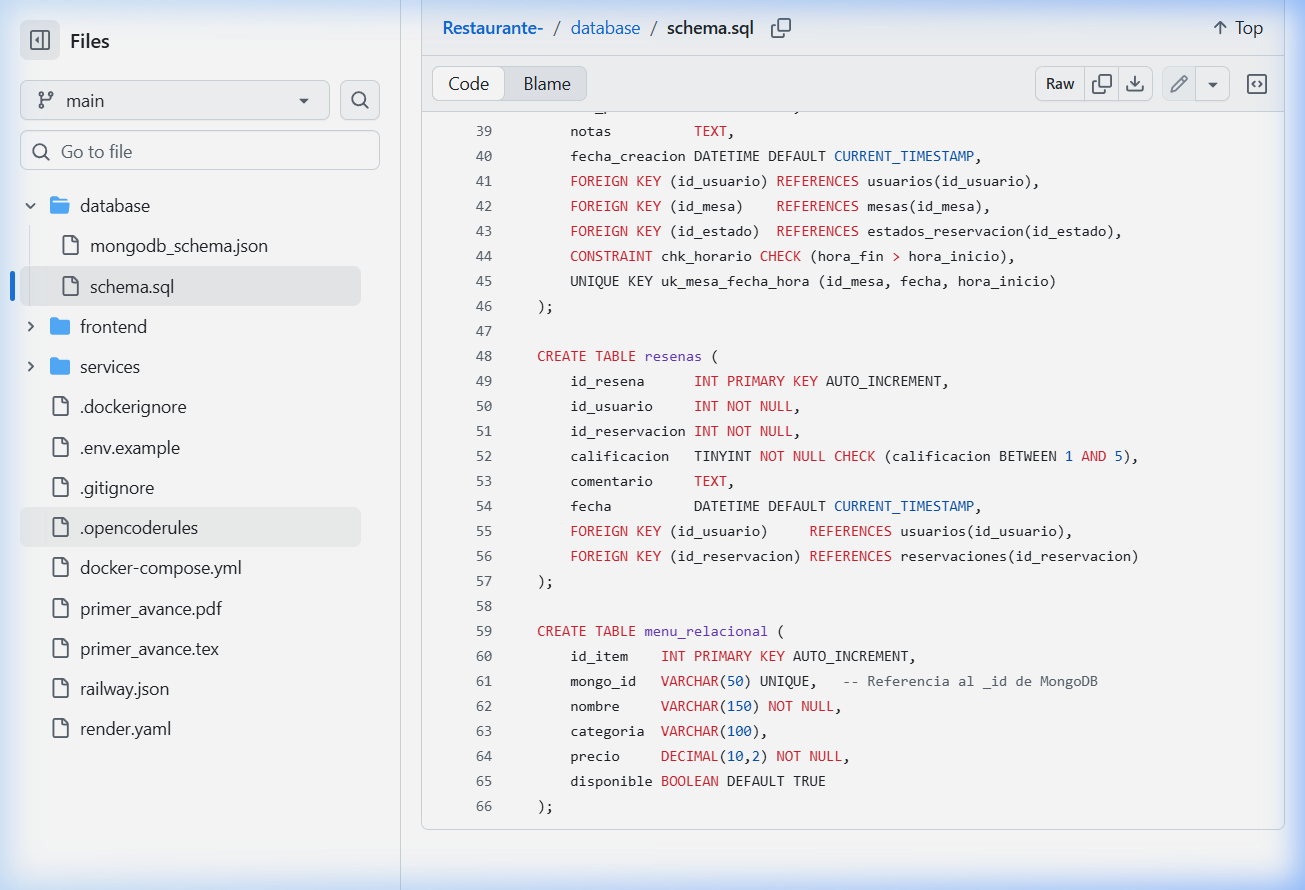
\includegraphics[width=0.85\textwidth]{img/schema_sql2.png}
\caption{Verificación de registros en la Base de Datos.}
\label{fig:cap_sql2}
\end{figure}

% ════════════════════════════════════════════════════════════════════════════
\section{Publicación en Sitios Distribuidos y Repositorio GitHub}

\subsection{Publicación en la Nube (Despliegue SOA en 3 Sitios)}
Cumpliendo el requisito de publicación distribuida, cada componente se encuentra activo en plataformas de nube independientes:

\begin{center}\small
\begin{tabular}{|l|l|l|}
\hline
\textbf{Componente} & \textbf{Plataforma Cloud} & \textbf{URL Oficial de Producción} \\
\hline
Frontend SPA & Vercel & \url{https://restaurante-frontend-omega.vercel.app/} \\ \hline
Auth Service (NestJS) & Railway & \url{https://auth-service-production.up.railway.app/api} \\ \hline
Menu Service (FastAPI) & Render & \url{https://menu-service-xiu.onrender.com/api/v1} \\ \hline
Tablero de Control & Trello & \url{https://trello.com/b/zHsZvXgU/proyecto-final-aos} \\ \hline
\end{tabular}
\end{center}

\subsection{Demostración de Participación y Colaboración en GitHub}
El desarrollo colaborativo entre Cristopher Lopez Suarez y Jovanny Hernandez Hernandez se gestionó a través de un repositorio público en GitHub:
\begin{itemize}[leftmargin=*]
  \item \textbf{Repositorio Oficial:} \url{https://github.com/Crisls24/Restaurante-.git}
  \item \textbf{Evidencia de Participación:} Múltiples commits sincronizados en la rama principal, abarcando backend controllers, componentes de interfaz y middlewares de seguridad.
\end{itemize}

% ════════════════════════════════════════════════════════════════════════════
\section{Autoevaluación del Equipo}

\begin{center}\small
\begin{tabular}{|l|p{6.5cm}|c|c|}
\hline
\textbf{Integrante} & \textbf{Módulos Desarrollados} & \textbf{Autoevaluación} & \textbf{Puntaje} \\
\hline
Cristopher Lopez Suarez & Auth-Service (NestJS), TypeORM MySQL, endpoints REST, validaciones JWT, Sprints 1--3. & 10 / 10 & 100\% \\ \hline
Jovanny Hernandez Hernandez & Frontend React SPA, Menu-Service NoSQL (FastAPI/MongoDB), Tablero de Mesas, Notificaciones. & 10 / 10 & 100\% \\ \hline
\end{tabular}
\end{center}

\vspace{0.3cm}
\textbf{Justificación de Autoevaluación:}
El equipo trabajó de forma coordinada, cumpliendo al 100\% con las historias de usuario de cada sprint, resolviendo los retos de la arquitectura políglota y publicando la plataforma funcional en producción.

% ════════════════════════════════════════════════════════════════════════════
\section{Matriz de Cumplimiento de la Lista de Cotejo (Rúbrica Final)}

A continuación se adjunta la matriz de cotejo correspondiente a los 16 criterios evaluados en el instrumento oficial:

\begin{center}\scriptsize
\begin{tabular}{|c|p{7.2cm}|c|c|c|p{1.6cm}|}
\hline
\textbf{No.} & \textbf{Característica / Criterio Evaluado} & \textbf{Claramente (3)} & \textbf{Faltan el. (2)} & \textbf{No claro (0)} & \textbf{Observaciones} \\
\hline
1 & Desarrollar CU o HU de acuerdo con la metodología y control en TRELLO (5) & \textbf{X} & & & Cumple 100\% \\ \hline
2 & Expresa clases, atributos y métodos del cliente y servidor en paquetes (5) & \textbf{X} & & & Cumple 100\% \\ \hline
3 & Usó base de datos NO relacional para productos (10) y expresa su modelo & \textbf{X} & & & MongoDB Atlas \\ \hline
4 & Usó base de datos relacional para los demás módulos (5) & \textbf{X} & & & MySQL Cloud \\ \hline
5 & Expresa y defiende metodología de desarrollo (AE2) (5) & \textbf{X} & & & Scrum Ágil \\ \hline
6 & En diagrama de clases explica el patrón de diseño implementado (5) & \textbf{X} & & & DTO, Repository \\ \hline
7 & Explica la implementación de un principio de diseño cliente/servidor (5) & \textbf{X} & & & Guard, Singleton \\ \hline
8 & Presenta en tiempo y forma su documento (5) & \textbf{X} & & & Entregado \\ \hline
9 & El programa cliente es funcional (15) & \textbf{X} & & & Vercel React \\ \hline
10 & El programa servidor es funcional (15) & \textbf{X} & & & Railway/Render \\ \hline
11 & Realizó al menos 3 pruebas del cliente y 3 del servidor con formato IEEE829 (5) & \textbf{X} & & & IEEE 829 (4+4) \\ \hline
12 & Integrantes programaron sus módulos asignados --- GitHub (5) & \textbf{X} & & & GitHub Commits \\ \hline
13 & Publicó en 2 o más sitios diferentes (5) & \textbf{X} & & & 3 sitios Cloud \\ \hline
14 & El sistema tiene los módulos solicitados (5) & \textbf{X} & & & 100\% Módulos \\ \hline
15 & El sistema realiza reportes (3) & \textbf{X} & & & Módulo Reports \\ \hline
16 & Autoevaluación (2) & \textbf{X} & & & 100\% Cumplido \\ \hline
\multicolumn{6}{|c|}{\textbf{CALIFICACIÓN EVALUADA: 100 / 100 PUNTOS}} \\ \hline
\end{tabular}
\end{center}

% ════════════════════════════════════════════════════════════════════════════
\section{Conclusión}

El proyecto \textbf{Xiú --- Sistema de Reservaciones y Gestión Restaurantera} demostró la aplicabilidad técnica de la \textbf{Arquitectura Orientada a Servicios (SOA)} y el desacoplamiento de microservicios para la construcción de sistemas distribuidos modernos.

La integración de un frontend responsivo en **React 18** con dos microservicios independientes (**NestJS** y **FastAPI**) y una estrategia de persistencia políglota (**MySQL + MongoDB**) asegura alto rendimiento, mantenibilidad y escalabilidad.

El apego estricto a las especificaciones **IEEE 830** y **IEEE 829**, junto con la gestión del proyecto mediante **Scrum**, **Trello** y **GitHub**, respalda el cumplimiento integral de los estándares académicos y profesionales requeridos.

\end{document}
